\fancyChapter{Conclusion}[]

This dissertation captures a novel way of answering the question "\textit{What is the purpose of perception}?". This was motivated in part by how I recall being first taught about perception --- bundled in a chapter alongside "sensation" --- a lesson all about the raw visual input to the retina and how the core properties of color, contrast, orientation, motion, and depth are processed in the brain. And although this was all interesting enough (particularly from a cellular or neurological perspective), none of these textbook properties involved how processing a static scene can also entail interacting with elements of \textit{time}. 

The purpose of this dissertation was thus to demonstrate empirically that when given certain types of static scenes, the mind does not only process static properties. Instead, it is important for the mind to represent the ongoing dynamics \textit{underlying} the scene --- whether it is the critical steps of how the scene came to be, or what is likely about to unfold next. This is the richness of visual processing: it forms these representations as a part of \textit{seeing what actually matters} in the world around us.

In a sense, the case studies presented here span how the mind can spontaneously recover important information about different moments in time: the \textit{past} (Chapters \ref{chap:PsychSci2023} \& \ref{chap:casual_hist}), where perception recovers the necessary causal history according to intuitive physics;  the \textit{present} (\Cref{chap:PsychSci2023}) where perception discounts superfluous scene details (of the non-informative, non-structural cloth folds) according to intuitive physics and recovers the important structural elements; and the \textit{future} (\Cref{chap:JEPG2024}), where afforded navigable paths are mentally traced for likely future traversal.  These dynamic representations --- recovering the past, prioritizing important deep structures in the present, and projecting into the future --- collectively demonstrate that visual processing extends far beyond merely parsing what is immediately present in the local, current environment. 

In the final section of this dissertation, I discuss some of my broader empirical work beyond these case studies, theoretical limitations and considerations, and the implications of each chapter for their broader fields.

%%%%%%%%%%%%%%%%%%%%%%%%%%%%%%%%%%%%%%%%%%%%%%%%%%%%%%%%%%%%%%%%%%%%%%%%%%%
\section{Seeing the Future: Intuitive Physics}\label{sec:stability_cfs}
%%%%%%%%%%%%%%%%%%%%%%%%%%%%%%%%%%%%%%%%%%%%%%%%%%%%%%%%%%%%%%%%%%%%%%%%%%%
Chapters \ref{chap:PsychSci2023} and \ref{chap:casual_hist} have both suggested that visual processing of intuitive physics forms dynamic representations of the \textit{past}.  In current ongoing work with collaborators \parencite{wong_unconscious_2024}, we further demonstrate that (a) intuitive physics is so foundational that it not only emerges in visual processing, but also that certain physical properties are \textit{prioritized even without awareness}, and (b) that intuitive physics enables us to form dynamic representations of the probable immediate \textit{future}.  

\begin{figure}[ht]
    \centering
    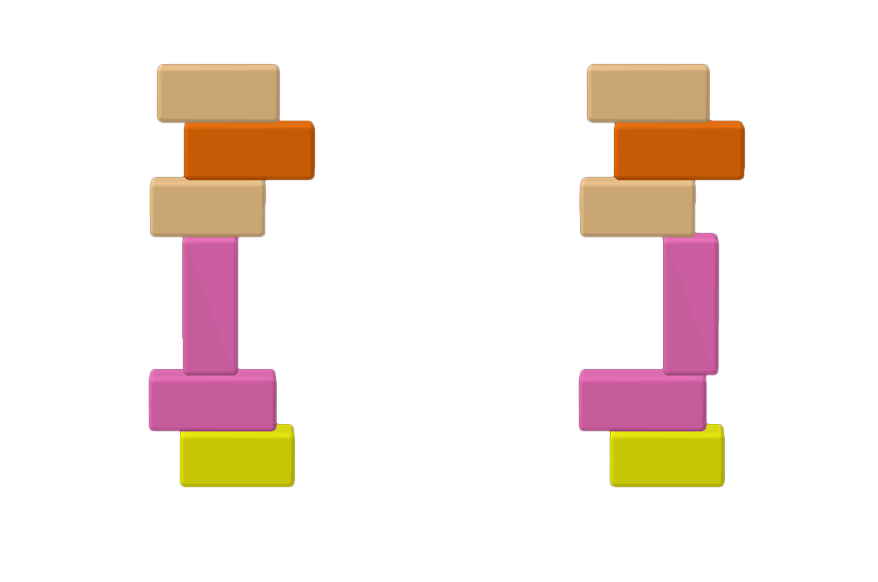
\includegraphics[width=\textwidth]{figures/DiscussFigs/stableunstable-pink.png}
    \caption
    {\textit{An unstable tower and its corresponding stable tower}. Stimuli pairs were generated by shifting the position of only one block, all while maintaining the convex hull of the tower.}
    \label{fig:DiscussFig_1}
\end{figure}

Observers viewed block towers --- some stable, some unstable --- defined in terms of whether they would collapse as a result of external physical forces (such as gravity) alone, as in the leftmost vs.~rightmost tower in \cref{fig:DiscussFig_1}.  We used an interocular suppression method called Continuous Flash Suppression (CFS; \cite{tsuchiya_continuous_2005}; see \cite{stein_breaking_2019} for a review) to render the towers initially invisible: observers viewed them monocularly through a mirror haploscope, while a dynamic Mondrian mask was presented to their other eye. We then measured how long towers took to break through this interocular suppression, as observers indicated when they became visually aware of anything other than the mask.  The results were clear and striking: unstable towers broke into visual awareness faster than stable towers. And this held even while controlling for other visual properties --- e.g.~while contrasting pairs of stable vs.~unstable towers that share the same convex hull, differing only in the horizontal placement of a single block. 

\begin{figure}
    \centering
    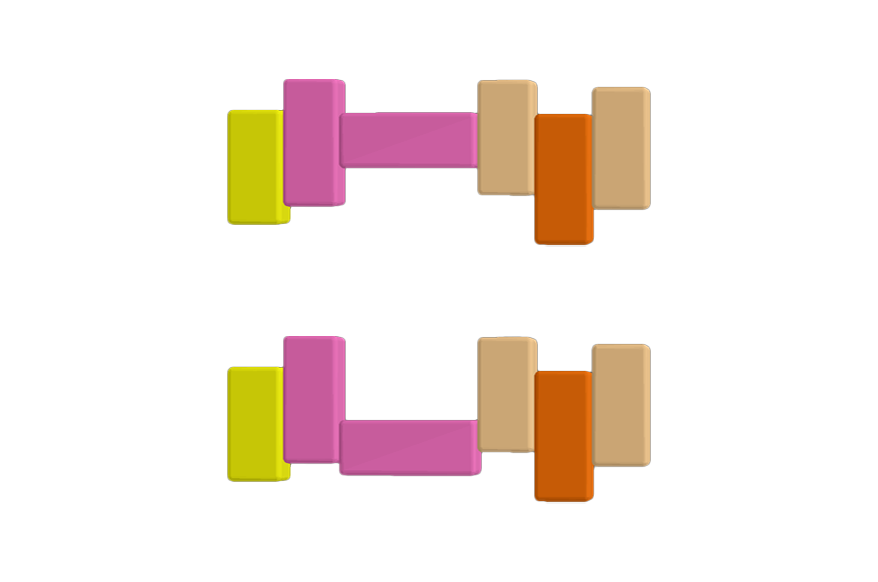
\includegraphics[width=\textwidth]{figures/DiscussFigs/stableunstable-pink2.png}
    \caption
    {\textit{An unstable tower and its corresponding stable tower, rotated 90 degrees}.}
    \label{fig:DiscussFig_1sideways}
\end{figure}

This difference in suppression breakthrough time disappeared when the towers were simply turned 90 degrees (as in \cref{fig:DiscussFig_1sideways}), reflecting that this was indeed an effect that emerged as a result of intuitive physics processing how gravity acts upon the block towers. Taken together, these results show that certain physical regularities are not just processed, but also visually \textit{prioritized} --- as when a tower is about to fall. The extraction of stability can occur not only through conscious deliberation, but also as an unconscious visual reflex \parencite{wong_unconscious_2024}.

Critically, this is yet another a demonstration of how we see \textit{what’s about to happen} --- beyond the path tracing in \Cref{chap:JEPG2024}.  Even though the raw visual input itself is just a single static image, we seem to be constructing dynamic representations of the critical information at hand: will the tower fall?  

%%%%%%%%%%%%%%%%%%%%%%%%%%%%%%%%%%%%%%%%%%%%%%%%%%%%%%%%%%%%%%%%%%%%%%%%%%%
\section{Seeing Unfinishedness: What Didn’t Happen}
%%%%%%%%%%%%%%%%%%%%%%%%%%%%%%%%%%%%%%%%%%%%%%%%%%%%%%%%%%%%%%%%%%%%%%%%%%%
In recent work with collaborators, we also consider yet another direction to explore visual representations of the future: specifically, do we detect when the future is \textit{not fulfilled}?  Or in other words, do we form dynamic representations of what has \textit{yet} to happen?  To answer these questions, we empirically examined the idea of “unfinishedness”.  

Unfinished tasks — from half-written papers, to interrupted dinner preparations --- tend to occupy our thoughts.  They can do so in a persistent (sometimes even frustrating) way, which seems specific to unfinishedness: the not-yet-started dinner seems of lesser concern, and the completed dinner is often already on its way to being forgotten — but when half-completed, the same tasks become especially mentally prominent. 

This phenomenon was first explored empirically in the 1930s, in the “Zeigarnik effect” \parencite{ellis_finished_1938}.  Subjects were instructed to complete various tasks, but were interrupted by an experimenter and kept from completing some of them.  Afterwards, subjects were asked to recall as many tasks as they could, and those left unfinished were more likely to be remembered.  This was attributed to a “state of tension” (p. 300) that arises when an interruption keeps us from finishing tasks (see also \cite{baddeley_zeigarnik-like_1963}; for a contemporary review, see \cite{macleod_zeigarnik_2020}).  And this “state of tension” has far-reaching consequences: unfinished tasks reduce cognitive flexibility \parencite{freeman_dont_2010}, impair sleep \parencite{syrek_unfinished_2014}, and reduce competence and work satisfaction \parencite{weigelt_finding_2019}.  This so-called “Zeigarnik Effect” has been previously explained by appeal to higher-level social motivations, e.g.~the weight of obligation or the salience of goals \parencite{eitam_motivated_2013, ferguson_mind_2013}, but my collaborators and I have shown that simple forms of unfinishedness are also spontaneously prioritized even in visual perception itself.  

Observers viewed simple animations of a path that gradually unfolded through a 2D maze, in the form of a simple line that moved from a salient ‘startpoint’ to an ‘endpoint’ (the small discs in \cref{fig:DiscussFig_2}).  As the path unfolded, probes (the colored squares in \cref{fig:DiscussFig_2}) appeared at haphazard times, and observers later reproduced the probes’ positions. Critically, the unfolding path sometimes reached its endpoint (‘finished’), or sometimes stopped shortly before this point (‘unfinished’).  Thus, observers experienced unfinishedness that was \textit{visual} (rather than cognitive), \textit{passive} (rather than active), and \textit{spontaneous} (rather than embedded in semantically-laden tasks and obligations).  
\begin{figure}
    \centering
    \includegraphics[width=\textwidth]{figures/DiscussFigs/unfinishedness.pdf}
    \caption
    {\textit{Caricature of a trial}. Observers viewed an animation of a purple path gradually unfolding between a brown startpoint and endpoint.  Probes (colorful squares) appeared along the path at haphazard times, and afterwards observers simply reproduced the probes’ positions. The path could either stop stop shortly before the endpoint (‘unfinished’ trials), or reach the endpoint (‘finished’ trials).}
    \label{fig:DiscussFig_2}
\end{figure}

Although the manipulation of unfinishedness was entirely task-irrelevant, it nevertheless had a powerful influence: Observers had far better memories for probe locations on unfinished trials (Ongchoco et al., under review; \cite{ongchoco_unfinishedness_2023}).  This same pattern held across several different experiments, even while carefully controlling for various lower-level properties of the displays (such as the speed and duration of the dot's motion). And the effect also generalized across different types of displays (e.g.~also replicating when the moving dot left a visible trace).  

This work thus reveals how yet another surprisingly rich property is extracted as part of perception, demonstrating that we not only form dynamic representations of what is likely \textit{about to happen}, but also when those representations of the future \textit{fail to happen}.  

%%%%%%%%%%%%%%%%%%%%%%%%%%%%%%%%%%%%%%%%%%%%%%%%%%%%%%%%%%%%%%%%%%%%%%%%%%%
\section{Temporal Dilation of Static Objects due to Dynamic ‘Oddballs’}
%%%%%%%%%%%%%%%%%%%%%%%%%%%%%%%%%%%%%%%%%%%%%%%%%%%%%%%%%%%%%%%%%%%%%%%%%%%

So much of this dissertation has been about time --- indirectly.  I’ve also explored time --- directly --- in work with collaborators \parencite{ongchoco_whats_2024}.  Chapters \ref{chap:PsychSci2023} \& \ref{chap:casual_hist} demonstrated that people recover the past even from seeing a static snapshot of the present.  In contrast, we here explored the opposite: how the context of the past can influence temporal perception of static objects in the present.  

Our experience of time is strikingly plastic: Depending on contextual factors, the same objective duration can seem to fly by or drag on (e.g.~\cite{eagleman_human_2008, grondin_timing_2010, matthews_time_2014}). For example, time seems to dilate (with durations seeming longer) when stimuli are more complex (e.g.~\cite{block_troubles_1978}), are less predictable (e.g.~\cite{pariyadath_brief_2008}), or contain more discrete events (e.g.~\cite{liverence_discrete_2012}) --- or even just when people are focusing on the passage of time in the first place (e.g.~\cite{macar_controlled_1994}).  Perhaps the most direct demonstration of such subjective time dilation is the \textit{oddball effect}: when seeing identical objects appear one after another, followed by an “oddball” (e.g., a disc that suddenly grows in size, in a sequence of otherwise static discs), observers experience this oddball as having lasted longer than its non-oddball counterparts (e.g., \cite{tse_attention_2004}). 

Despite extensive work on this phenomenon, a surprisingly foundational question remains unasked: What actually gets dilated? Beyond the oddball, are the objects just before (or just after) the oddball also dilated? As in previous studies, observers viewed sequences of colored discs, one of which could be the oddball --- and subsequently reproduced the oddball’s duration. Unlike previous studies, however, there were also critical trials in which observers instead reproduced the duration of the disc immediately before or after the oddball. A clear pattern emerged: oddball-induced time dilation extended to the post-oddball disc, but not the pre-oddball disc. Whence this temporal asymmetry? We suggest that an oddball’s sudden appearance may induce uncertainty about \textit{what will happen next}, heightening attention until after the uncertainty is resolved.



%%%%%%%%%%%%%%%%%%%%%%%%%%%%%%%%%%%%%%%%%%%%%%%%%%%%%%%%%%%%%%%%%%%%%%%%%%%
\section{On Evolution \& Developmental Approaches}
%%%%%%%%%%%%%%%%%%%%%%%%%%%%%%%%%%%%%%%%%%%%%%%%%%%%%%%%%%%%%%%%%%%%%%%%%%%

\textit{Why} do Chapters \ref{chap:PsychSci2023}-\ref{chap:JEPG2024} so consistently find dynamic representations of time, far beyond what the static image itself depicts?  In part, I believe the phenomena discussed here (intuitive physics, causal history, navigational affordances) can be explained partially by way of evolutionary importance.  

Take navigational affordances, for example.  When you are in a new environment, perhaps one of the most critical questions to answer is “how do I get out of here?”  In a forest, there are trees and brambles blocking the paths, or some routes (e.g.~on a rainy day) are way more slippery to traverse than others.  When the presence of a predator is detected, there is little time to retroactively appraise the environment --- as immediate action is necessary.  Or in a cave, there is a constant awareness of the shortest path out, and if that exit gets blocked.  In this way, processing navigational affordances would be essential for determining how to escape --- and whether escape is even possible at all. 

In the case of causal history, seeing a bitten fruit on the side of the road provides important information of possible forces at play in a given environment (in this case, the presence of an agent that can bite).  Alternatively, seeing a pile of smashed fruit can give information on some object (or agent) with great blunt force being present.  Or consider intuitive physics, particularly the perception of stability, as a structure that could collapse on top of you is inherently dangerous. Even on a smaller scale, a precariously placed glass vase requires action --- either to correct its positioning, or to avoid it before it falls.

In short, these properties could be so fundamental and critical to survival that it would be disadvantageous to take the time to learn them slowly over multiple experiences.  Do even young infants exhibit the ability to perceive these rich properties relevant for both the past and the future of a scene?  In this way, it seems there could be great potential synergy between the topics here and developmental approaches, which could lend insight on how and whether sensitivity develops over time.  

Of course, plenty of hallmark studies in developmental psychology have already focused specifically on physics reasoning in children (see \cite{spelke_precis_2024}, for a review).  For example, various classic studies have demonstrated that infants are sensitive to physical principles such as gravity and support, showing surprise when objects appear to violate these constraints (e.g., \cite{baillargeon_development_1992, hespos_reasoning_2001,stahl_observing_2015}). Similarly, work on violations of object permanence and cohesion shows that infants expect objects to behave according to principles of persistence (see \cite{baillargeon_innate_2008}, for a review).  This literature has even expanded to include infant reasoning about the intuitive physics of non-rigid substances, with studies demonstrating that they can distinguish between solids and liquids based on their physical properties \parencite{hespos_five-month-old_2009}, that they have expectations for how liquids flow and fill containers (see \cite{hespos_physics_2012}), and that they understand basic principles of substances like sand \parencite{hespos_five-month-old_2016}.  

On the other hand, work on affordances and causal history in children is surprisingly relatively limited. Gibson's classic visual cliff studies do capture children's seemingly innate sensitivity to navigational affordances: infants perceive depth and hesitate to crawl over a drop-off well before they have significant experience with falling \parencite{gibson_visual_1960}. Since then, there has been a variety of work on cliffs (see \cite{adolph_infants_2012} for a review) and slopes (e.g.~\cite{adolph_crawling_1993}).  One study examined affordances of apertures (tight spaces to fit through), demonstrating that infants can successfully do so, but mainly when it would be dangerous to fail \parencite{franchak_what_2012}.  Meanwhile, the traversability of obstacles or barriers seems to depend more on a toddler’s specific walking experience rather than general walking skill development \parencite{kingsnorth_walking_2000}.  So although there are good roots of research on how children process navigational affordances, there are many open questions remaining, especially when compared to the greater range of developmental literature on intuitive physics.  For instance, how might children approach multiple paths, other kinds of dangerous terrain types beyond cliffs, or even how do they remember scenes with different affordances available (or not available at all)?  This gap is particularly notable given how important navigational affordances would be for survival from an evolutionary perspective.

And to my knowledge, there exists only one instance of causal history being assessed developmentally at all.\footnote{I will also mention that there is an additional recent study asked children (4-8 years old) to reproduce a block tower that is presented to them by Landau and colleagues (\citeyear{landau_young_2024}).  Children built the towers bottom-to-top, in a layer-based fashion, similar to that of adults.  Notably, children did not seem to “experiment” with the possibility of building top-to-bottom, meaning that this behavior is in line with what would be expected from extracting causal history as guided by necessary intuitive physics.  However, because it is a reproduction task, the physics constraints (even without causal history processing) would have resulted in the same behavioral pattern and therefore I cannot say this is a developmental study demonstrating causal history knowledge.} Goulding and colleagues (\citeyear{goulding_time_2025}) examined how children infer temporal order from a variety of images, including static images of a stack of hats or a tower of ice cream scoops. Children (by age 5) are able to judge the placement order of these vertically stacked objects when explicitly asked questions like "What came first?" or "What came last?", though younger children (aged 3-4) seem less adept. This aligns with the intuitive physics-based causal history explored in \Cref{chap:casual_hist}, suggesting that even young children can understand the necessary temporal constraints imposed by physical laws like gravity and support. It remains to be developmentally assessed via other methods beyond direct questions.



The current adult-focused paradigms in Chapters \ref{chap:PsychSci2023}-\ref{chap:JEPG2024} cannot directly address the question of evolutionary importance for intuitive physics, causal history, or affordances.  Adapting these ideas and questions for developmental populations could provide valuable insights into how (and whether) foundational mechanisms emerge to process these rich dynamic representations.

%%%%%%%%%%%%%%%%%%%%%%%%%%%%%%%%%%%%%%%%%%%%%%%%%%%%%%%%%%%%%%%%%%%%%%%%%%%
\section{Further Considerations on the Limitations of Time}
%%%%%%%%%%%%%%%%%%%%%%%%%%%%%%%%%%%%%%%%%%%%%%%%%%%%%%%%%%%%%%%%%%%%%%%%%%%
While this dissertation has demonstrated how visual processing of certain static images can entail rich, dynamic representations of both probable past states and future states, it's important to consider the temporal limits of these representations. Although the studies presented here don't empirically explore these boundaries, theoretical considerations suggest some inherent constraints on how far these dynamic representations can extend (in either temporal direction).
 
Consider a simple scene of a ball rolling down a ramp.  How far into the future might our visual system represent its trajectory?  While we might be tempted to imagine an unlimited temporal scope, both computational and practical constraints suggest otherwise.  From a computational perspective, representing extended temporal sequences would quickly become intractable, especially in real-world scenes containing multiple interacting objects.  Each additional object would exponentially increase the number of possible future states that would need to be represented, quickly overwhelming any reasonable processing capacity.  Just take any maze or obstacle scene from \Cref{chap:JEPG2024}, for example.  There are only two probes that participants are tasked with tracking, and there’s one afforded path between them.  What if four probes?  The scene now not only consists of 4 separate objects, but also each of those 4 objects has 3 different target probes, each with a different possible path to navigate in the future.
 
Moreover, the utility of extended temporal representations diminishes rapidly. In our ball-and-ramp example, the most relevant future states might include the ball reaching the bottom of the ramp and coming to rest.  Representing the state of the scene hours or days into the future would provide little additional value, and furthermore, the certainty of predictions decreases dramatically with time.  Take the vertically stacked blocks as in \Cref{chap:casual_hist}.  The representation of the past discussed in that chapter only concerns the (relatively) recent period while the tower is being constructed.  But even in theory, rolling back the clock even further (to the point that the blocks are just randomly strewn about the table, unstacked) provides little additional value either.  There are an infinite number of positions or locations those blocks could be strewn about in, before being picked up and assembled into the tower.  Environmental variables, external interventions, and accumulating uncertainties would render such long-term representations both computationally expensive and practically unreliable.
 
This suggests that our visual system likely operates within an optimal temporal window --- one that balances computational resources against practical utility. This window would be flexible, adapting to the specific properties and dynamics of the scene at hand.  In a study such as the one discussed in Section \ref{sec:stability_cfs}, a precariously unstable tower of blocks might elicit representations of imminent collapse, while a stable structure might generate more limited future-oriented representations.  Similarly, representations of past states likely extend only far enough to capture causally relevant history, rather than attempting to reconstruct an object's entire historical trajectory.  Given this scene-based variability, the work here cannot (and arguably \textit{should not}) offer information on the specific temporal constraints. 

%%%%%%%%%%%%%%%%%%%%%%%%%%%%%%%%%%%%%%%%%%%%%%%%%%%%%%%%%%%%%%%%%%%%%%%%%%%
\section{On Other Related Visual Phenomena}
%%%%%%%%%%%%%%%%%%%%%%%%%%%%%%%%%%%%%%%%%%%%%%%%%%%%%%%%%%%%%%%%%%%%%%%%%%%

Throughout this dissertation, I have treated its primary theme — the creating of intrinsically dynamic visual representations even from static scenes — as a largely novel discovery and perspective in vision science.  But of course there are other phenomena that seem related (if still different in critical ways).  Here I briefly discuss three of them: \textit{representational momentum},  \textit{serial dependence}, and  \textit{boundary extension}.  In studies of the well-known phenomenon of \textit{representational momentum} (see \cite{hubbard_representational_2005}), participants are shown a brief animation of a square (or object) moving forward for a few frames, and then later asked to report the last position of the square.  The position of the square is misremembered to be at a position "in the future", further forward than where the animation initially ended.  While this shares similarities with how observers seem to represent the possible future --- as in \Cref{chap:JEPG2024}, where observers formed dynamic representations of navigable future paths — the critical difference between representational momentum and the ideas presented throughout this dissertation is that the visual input triggering the dynamic underlying representation itself is not static. There's dynamic movement information that is being presented to the observer, from which they then continue to construct the likely future.  Meanwhile, the stimuli in the current experiments, such as cloth-covered objects or a scene of obstacles, for example, do not rely on preceding frames of animation to establish the dynamics.

In a similar vein, in the phenomenon of \textit{serial dependence} (see \cite{fischer_serial_2014}, for a review), participants’ reproductions of a tilted line’s orientation is influenced by the orientation of a gabor patch previously presented in the same spatial location.  But like representational momentum, serial dependence is different from the rest of the work in this thesis because it also relies on previously (recently) presented information to influence how current input is perceived.  These differences become especially salient when compared to the single trial experiments (such as Expt.~4 in \Cref{chap:casual_hist}, or Expt.~1 in \Cref{chap:PsychSci2023}). In such cases, participants merely saw a single image (of blocks stacked on a table, or of a cloth-covered object). There are no context-providing images that precede the image, unlike the sequence of movement frames in representational momentum, or the orientation-biasing gabor patches in serial dependence. In particular, because these were single trial studies where each participant only completes the task once, there was no possibility for cross-trial effects (where the participant may have learned what to expect, or have developed strategies to accomplish the task better).  Furthermore, serial dependence lacks the "past" or "future" element as introduced by causal history and affordances, instead only affecting perception of the present stimuli. I would additionally argue that it’s different even still from \Cref{chap:PsychSci2023} (which also concerns deeper representations of the present) as \Cref{chap:PsychSci2023} involves the dynamics of using intuitive physics to subtract out the cloth --- meanwhile, serial dependence does not seem to involve any dynamic reconstruction or simulation of the scenes, rather, it is merely that memory is biased towards recently shown information.

And finally, the phenomenon of \textit{boundary extension} captures how observers misremember a single snapshot of a scene, reproducing the scene with a wider angle or "zoomed out", as the boundary of the image is expanded (\cite{intraub_wide-angle_1989}; see \cite{hubbard_boundary_2010} for a review). Boundary  extension is often effectively demonstrated when the initial scene consists of objects that were partially cropped out, as participants reproduce the scene with a wide enough angle to draw in the whole, uncropped object.  At first glance, this seems to fit closely with the body work presented here, particularly because the initial input is just a static scene.  However, I currently know of no evidence that the process underlying boundary extension is dynamic.  Like serial dependence, it could be just that the scene is immediately misremembered as “wide angle”, not necessarily that there’s any form of a gradual “zooming out” process --- versus the clear unfolding processes of “rebuilding the tower according to physics” (\Cref{chap:casual_hist}), or “tracing along the paths” (\Cref{chap:JEPG2024}).  And additionally, boundary extension does not speak to forming representations of the past or the future.\footnote{In the review by Hubbard and colleagues (\citeyear{hubbard_boundary_2010}), they mention that work on how boundary extension interacts with representational momentum exists --- where participants were only given a single static image to remember (e.g. a galloping horse), instead of the usual series of images in typical representational momentum tasks.  This would have theoretically fit nicely with the idea of "representing the future", even from static images as proposed in this dissertation; however, they work they cite is a 2004 paper from the 45th Annual Meeting of the Psychonomic Society, of which there is no text, data, or stimuli that is currently accessible. I thus do not discuss their work here.}

In brief, this dissertation stands as a distinct demonstration not only of how even seeing certain static images results in dynamic representations, but also how these dynamic representations involve recovering more than just the present --- including the past, and the future. This framework is not intended to exclude future phenomena, as intuitive physics, causal history, and affordances are simply demonstrations of the overarching idea.


%%%%%%%%%%%%%%%%%%%%%%%%%%%%%%%%%%%%%%%%%%%%%%%%%%%%%%%%%%%%%%%%%%%%%%%%%%%
\section{Why This Matters}
%%%%%%%%%%%%%%%%%%%%%%%%%%%%%%%%%%%%%%%%%%%%%%%%%%%%%%%%%%%%%%%%%%%%%%%%%%%

Each of the empirical chapters presented here have contributed not only to new perspectives on how perception forms rich, dynamic representations, but also each contribute uniquely to their respective fields. 

Within intuitive physics, this work makes several key contributions. First, it moves beyond the more frequently studied types of physics --- involving rigid bodies --- and extends into soft materials, which have completely different internal dynamics. Second, at the time of its publication, it was the first demonstration of spontaneous visual processing of intuitive physics (as the task was neither directly asking about the intuitive physics in the scene, nor would performance on the task have benefited from intuitive physics).

Within causal history, the contributions are significant. First, given the scarcity of empirical work in this area, this research stands as the second empirical paper supporting perception of causal history. Second, while previous literature (including those using judgment-based tasks; e.g.~\cite{schmidt_visual_2019}, \cite{fleming_getting_2019}) focuses on object-focused transformations that distort the shape itself (e.g., being bitten, being twisted, being inflated, etc; \cite{chen_perception_2016}), this work introduces an entirely new category for a type of history: based on physics in the scene (e.g.~that items vertically stacked must have been built from the bottom up). Third, through this combination with intuitive physics, it enables discussion of causal history as existing in the \textit{relations between} objects, not just within singular objects that were subjected to some transformation as previous papers did.

Within affordances, this work makes important theoretical distinctions. First, it helps disentangle two elements of Gibson's influential theories that have often been conflated: (a) affordances as stimulus-driven percepts that are extracted in visual processing, even though they are more complex than other 'typical' low-level features of color and shape, and (b) the notion that affordances are perceived "directly" --- as a function of brute "resonance" with the environment, without intermediate inferential steps or symbolic representations \parencite{gibson_ecological_1979}. The research on maze-like stimuli and obstacle-filled scenes contributes to demonstrating the first critical idea of affordances while separating it from claims about direct perception. Second, it demonstrates that affordances can act upon a scene even when they're not relative to the body of the person itself (because the navigational affordances of the narrow paths in the maze would only accommodate the movement of probes, not the body of the observer).

Within visual routines, this research advances our understanding in multiple ways. First, it challenges a well-established implicit assumption in the field --- that visual routines need to be on-demand or task-driven \parencite{ullman_visual_1984} --- by showing that certain stimuli can invoke the operation of visual routines spontaneously. Second, it employs new kinds of ecological stimuli beyond those previously tested (which typically involved various simple bendy lines and probes placed along those lines).

In closing, what we see is more than just a visual collection of colors, shapes, and objects frozen in time. Although I doubt the opening chapters in vision textbooks will change anytime soon (because, of course, the basics are still essential), perhaps the \textit{way} researchers think about the purpose of perception will shift: It's not just "What's out there?", but rather the recovery of the underlying dynamics --- addressing "What's happening?" , "What happened?", and "What's about to happen?".
